\chapter{VLANs: Part 1}\label{vlans-part-1}

WHAT IS A LAN ?

\begin{itemize}
\tightlist
\item
  A LAN is a single BROADCAST DOMAIN, including all devices in that
  broadcast domain.
\end{itemize}

\section{Broadcast Domains}\label{broadcast-domains}

\begin{itemize}
\tightlist
\item
  A BROADCAST DOMAIN is the group of devices which will receive a
  BROADCAST FRAME (Destination MAC : FFFF.FFFF.FFFF) sent by any one of
  the members.
\end{itemize}

Image of LAN with FOUR BROADCAST DOMAINS (192.168.1.0 / 24)

\begin{figure}
\centering
\pandocbounded{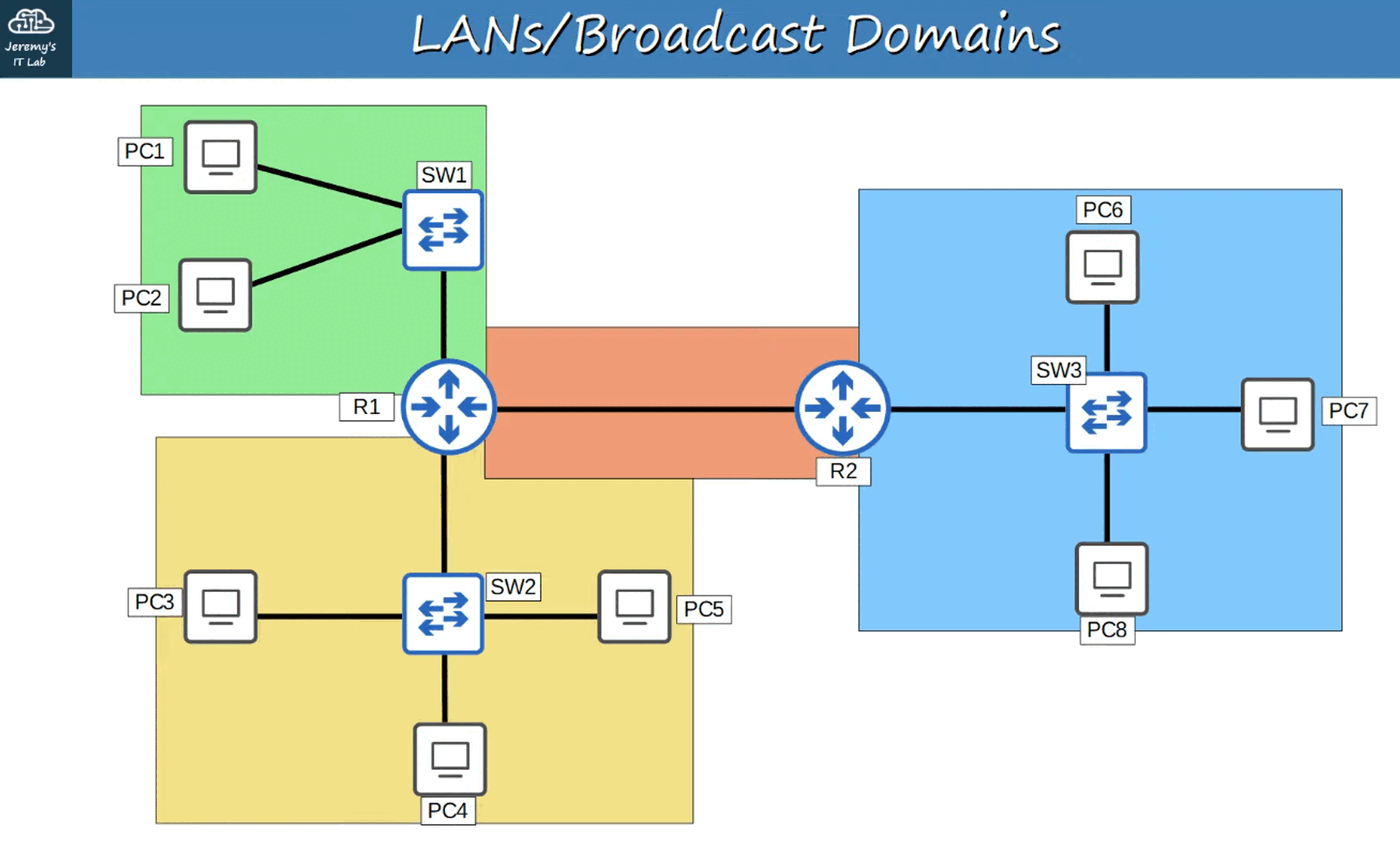
\includegraphics[keepaspectratio,alt={image}]{images/17-vlan-part1/img-001.png}}
\end{figure}

Performance :

Lots of unnecessary BROADCAST traffic can reduce network performance.

\begin{figure}
\centering
\pandocbounded{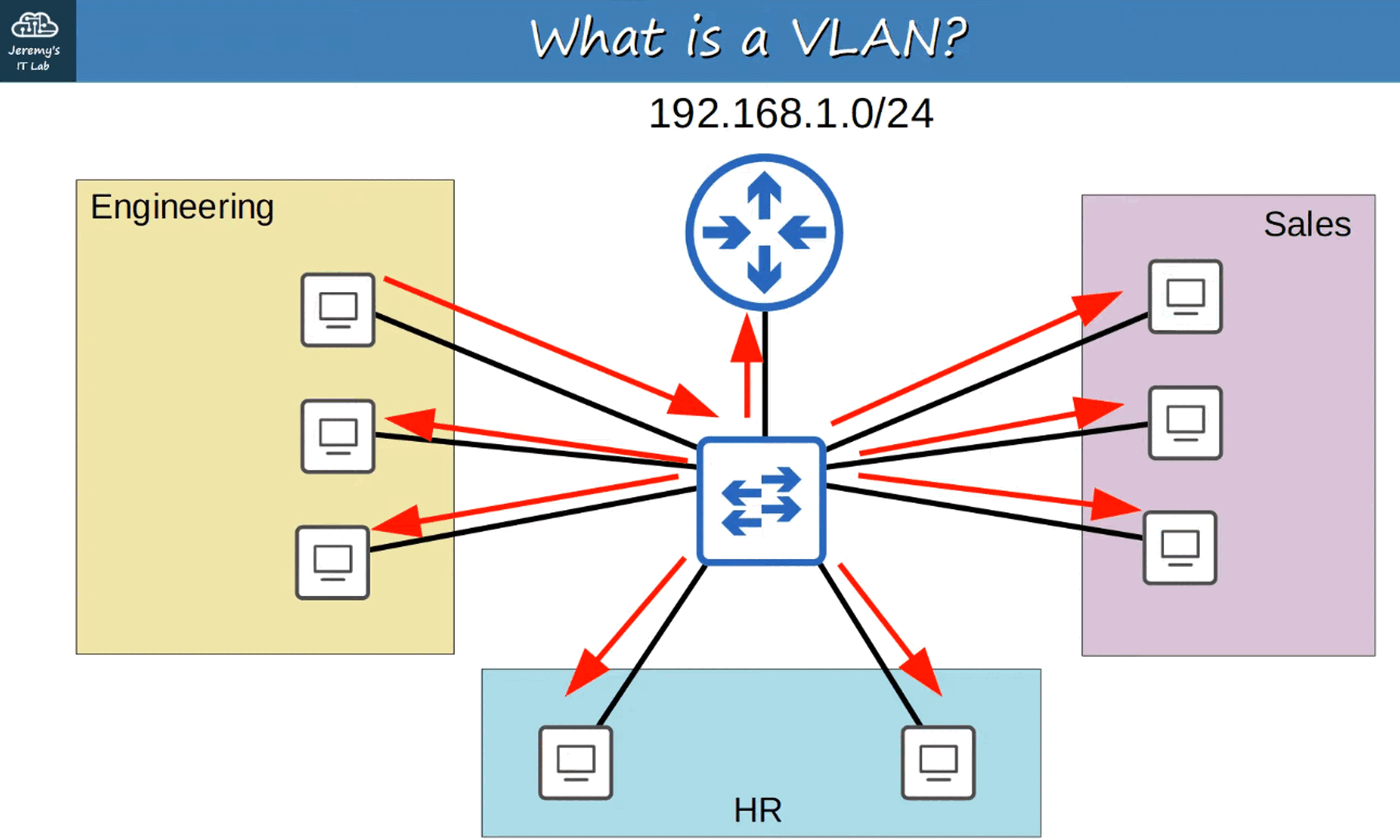
\includegraphics[keepaspectratio,alt={image}]{images/17-vlan-part1/img-002.png}}
\end{figure}

BROADCAST FRAME flooding all our subnets with unnecessary traffic.

\begin{figure}
\centering
\pandocbounded{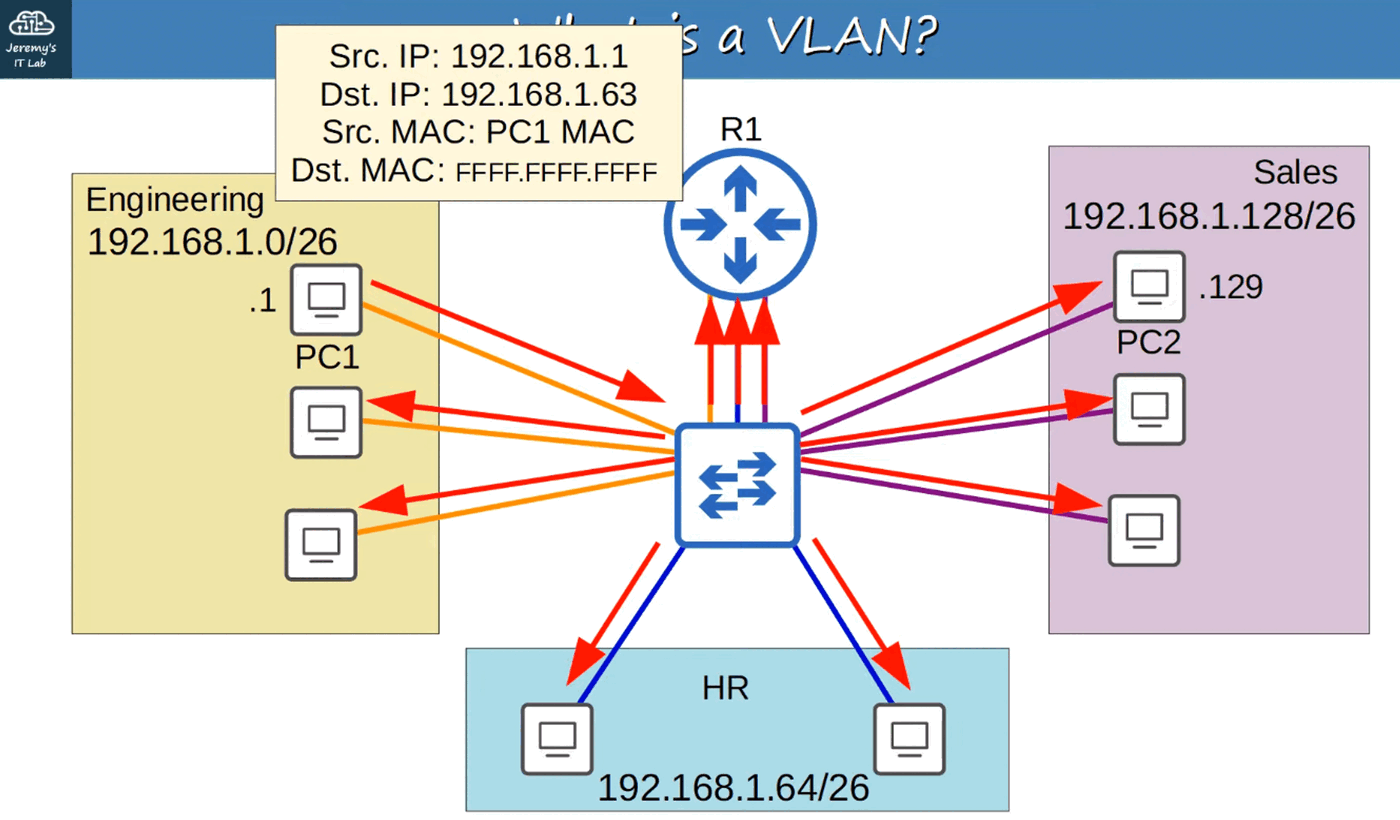
\includegraphics[keepaspectratio,alt={image}]{images/17-vlan-part1/img-003.png}}
\end{figure}

Security :

Even within the same office, you want to limit who has access to what.
You can apply security policies on a ROUTER / FIREWALL. Because this is
one LAN, PC's can reach each other directly, without traffic passing
through the router. So, even if you configure security policies, they
won't have any effect.

\begin{figure}
\centering
\pandocbounded{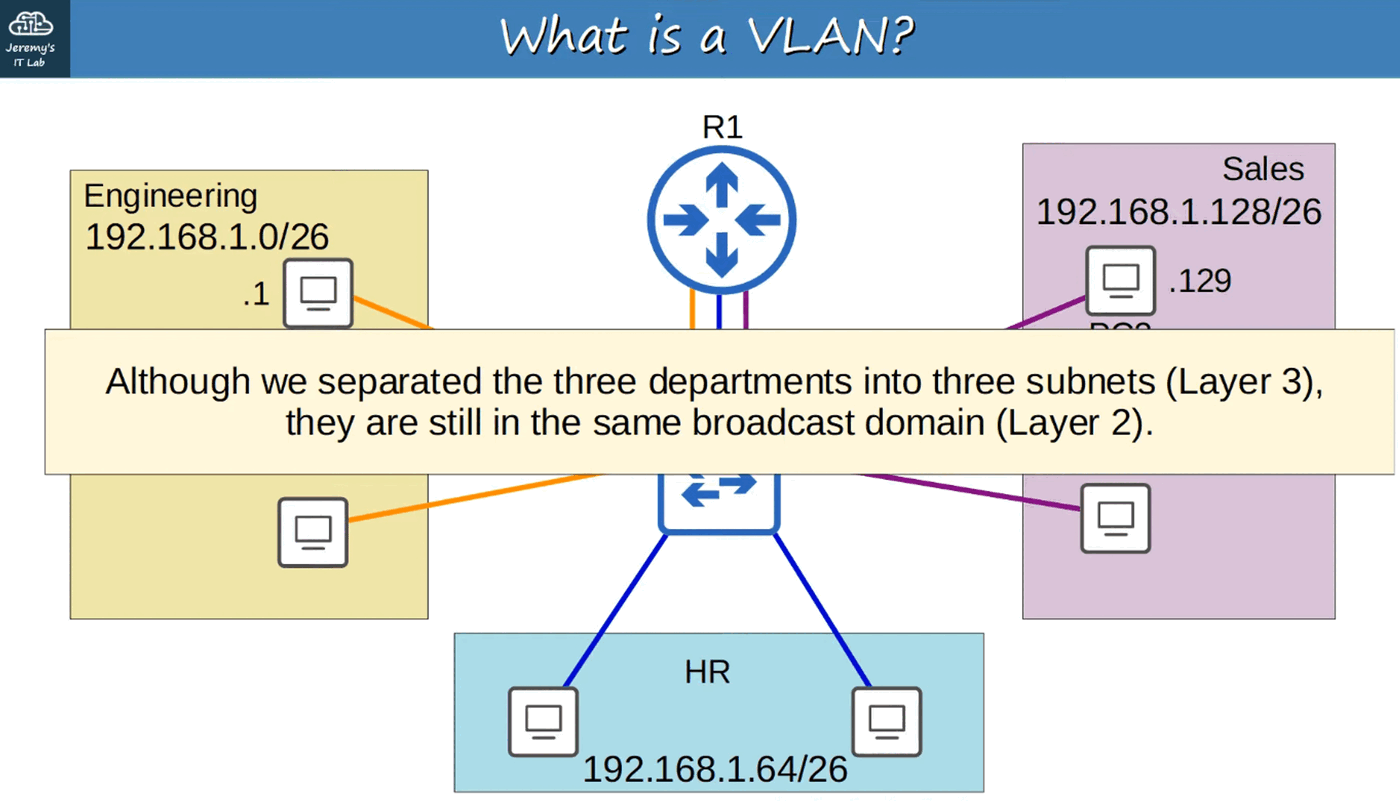
\includegraphics[keepaspectratio,alt={image}]{images/17-vlan-part1/img-004.png}}
\end{figure}

WHAT IS A VLAN ?

\section{VLANs}\label{vlans}

\begin{itemize}
\tightlist
\item
  logically separate end-hosts at LAYER 2
\item
  are configured on Layer 2 SWITCHES on a per-interface basis.
\item
  any END HOST connected to that interface is part of that VLAN
\end{itemize}

PURPOSE OF VLANs:

Network Performance :

\begin{itemize}
\tightlist
\item
  Reduce unnecessary BROADCAST traffic, which helps prevent network
  congestion, and improve network performance
\end{itemize}

Network Security :

\begin{itemize}
\tightlist
\item
  Limiting BROADCAST and unknown UNICAST traffic, also improves network
  security, since messages won't be received by devices outside of the
  VLAN
\end{itemize}

\begin{figure}
\centering
\pandocbounded{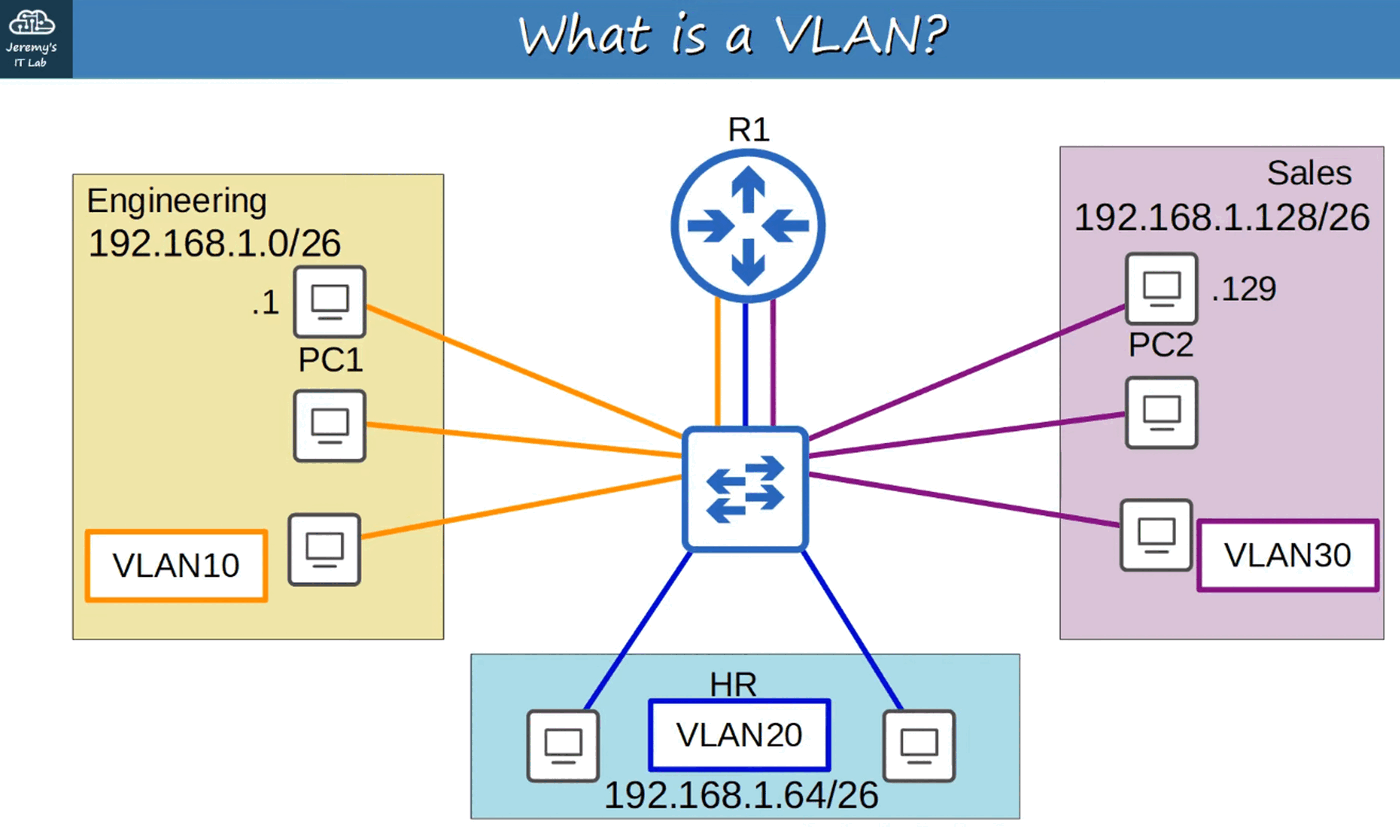
\includegraphics[keepaspectratio,alt={image}]{images/17-vlan-part1/img-005.png}}
\end{figure}

SWITCHES do not forward traffic directly between HOSTS in different
VLANS

\begin{figure}
\centering
\pandocbounded{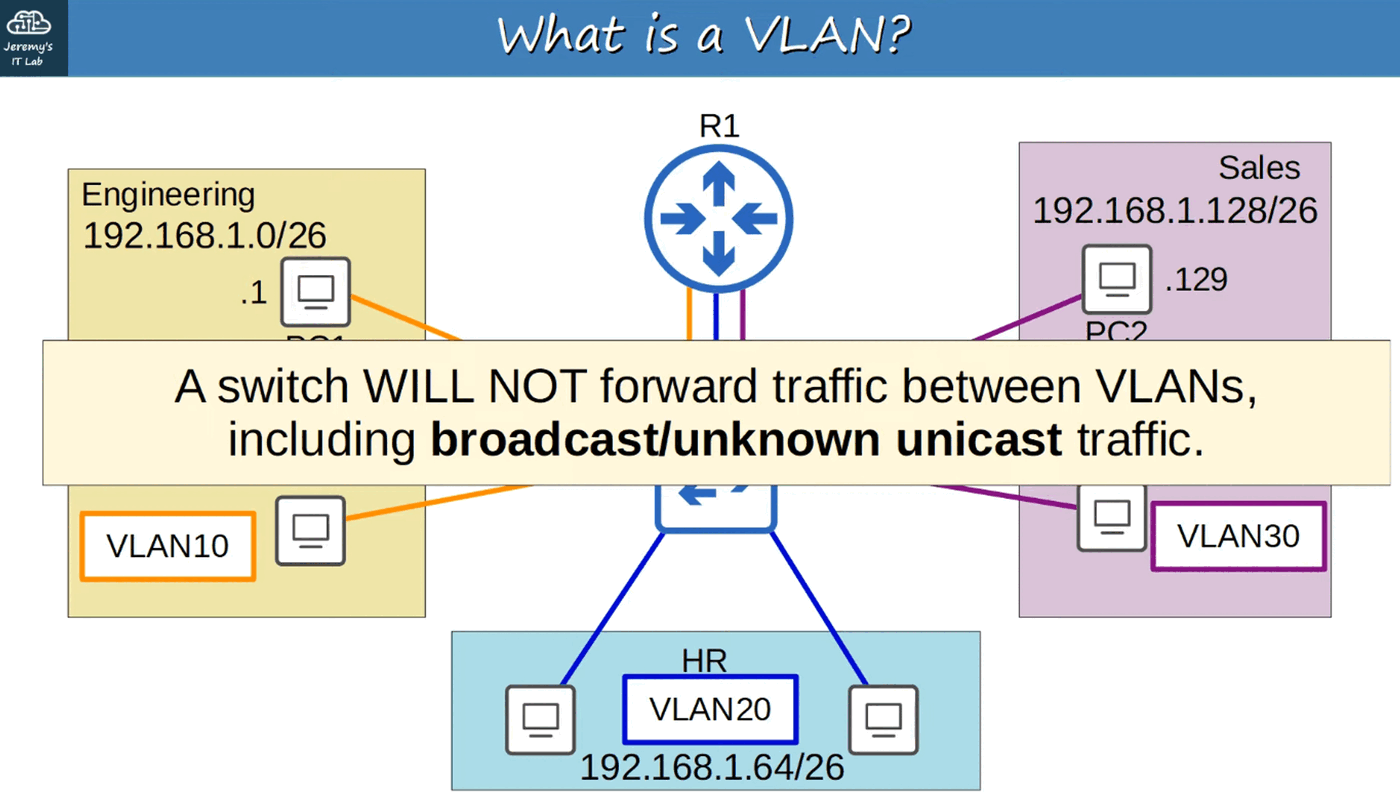
\includegraphics[keepaspectratio,alt={image}]{images/17-vlan-part1/img-006.png}}
\end{figure}

\begin{figure}
\centering
\pandocbounded{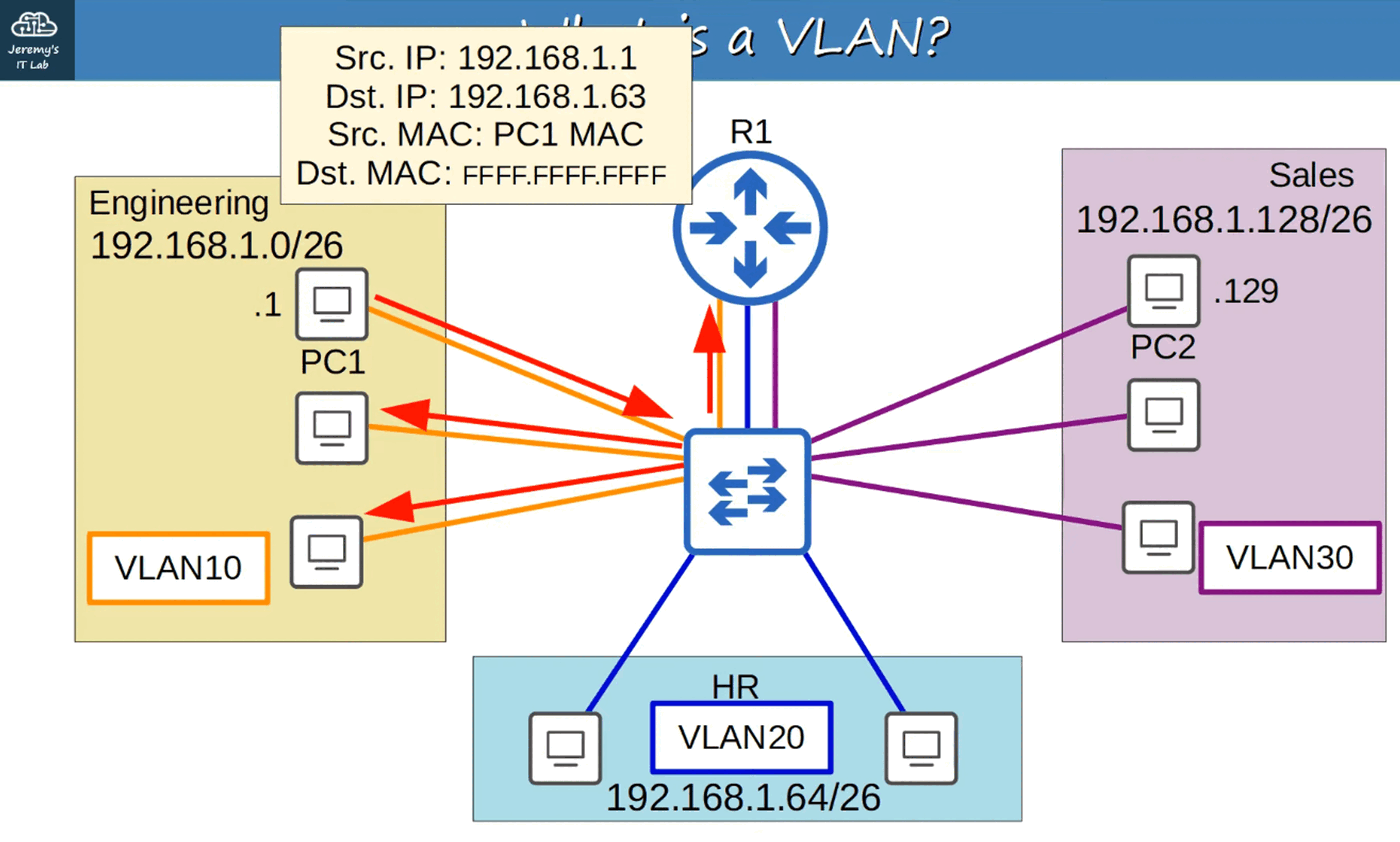
\includegraphics[keepaspectratio,alt={image}]{images/17-vlan-part1/img-007.png}}
\end{figure}

Sending Packets to another VLAN (Routed through R1)

\begin{figure}
\centering
\pandocbounded{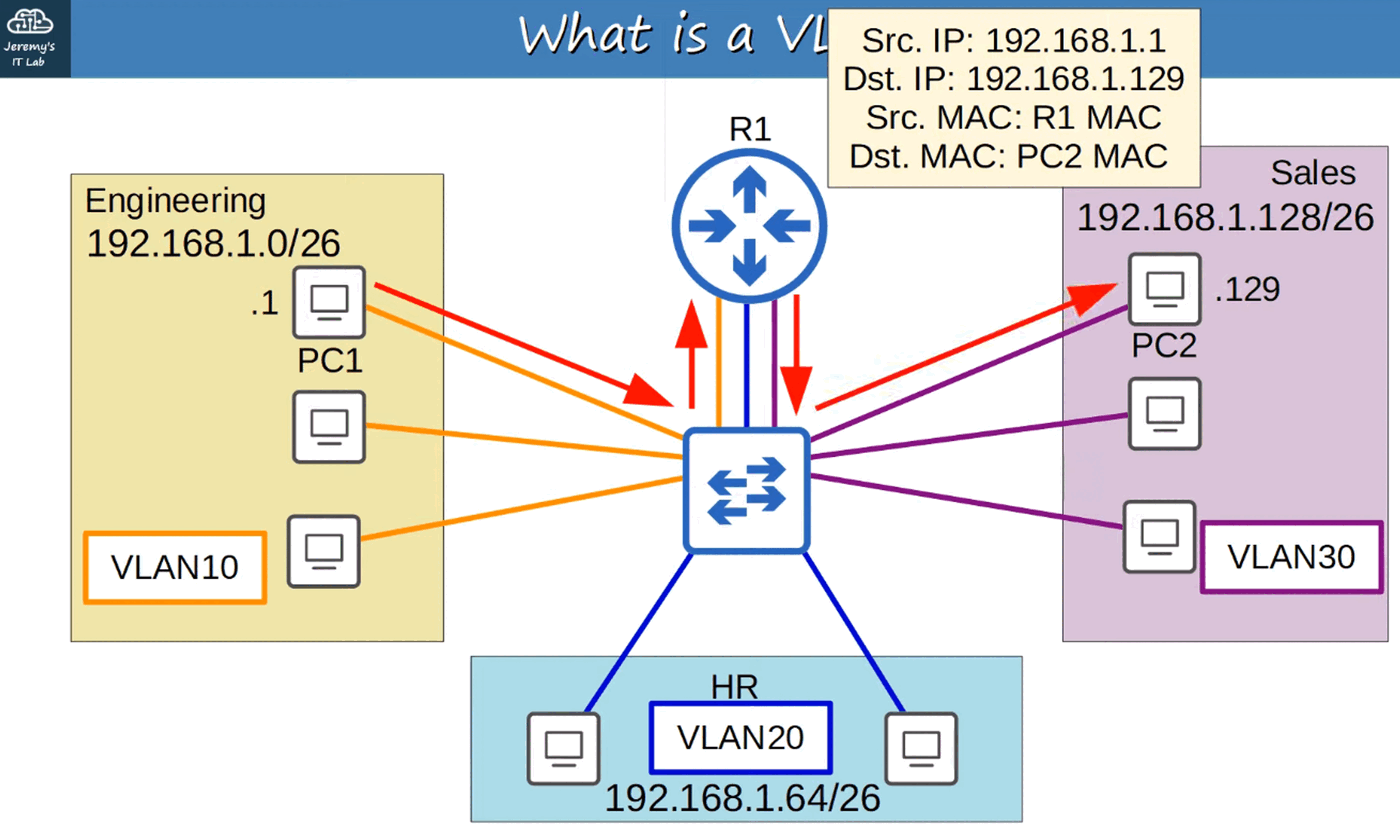
\includegraphics[keepaspectratio,alt={image}]{images/17-vlan-part1/img-008.png}}
\end{figure}

\begin{figure}
\centering
\pandocbounded{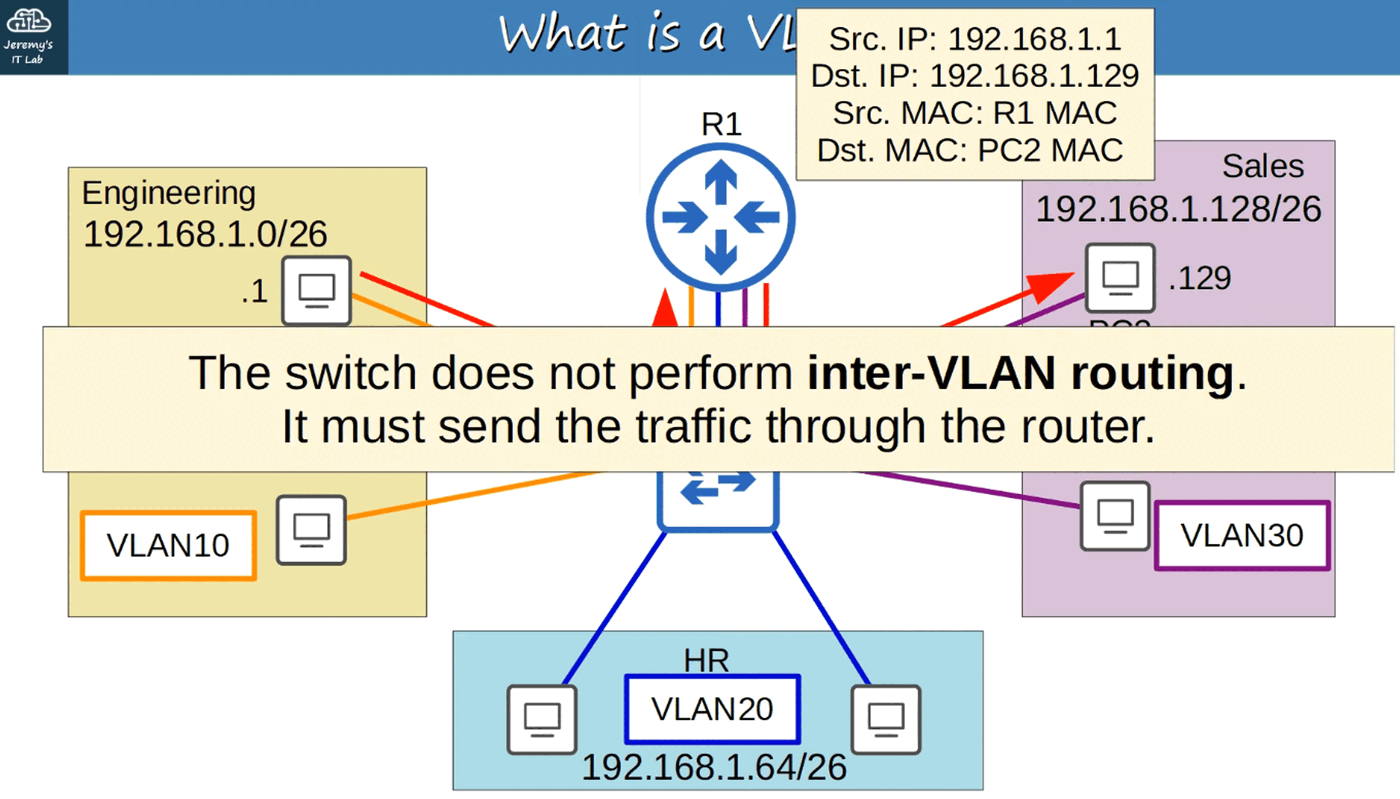
\includegraphics[keepaspectratio,alt={image}]{images/17-vlan-part1/img-009.png}}
\end{figure}

\section{How to Configure VLANs on Cisco
Switches}\label{how-to-configure-vlans-on-cisco-switches}

\#show vlan brief

\begin{figure}
\centering
\pandocbounded{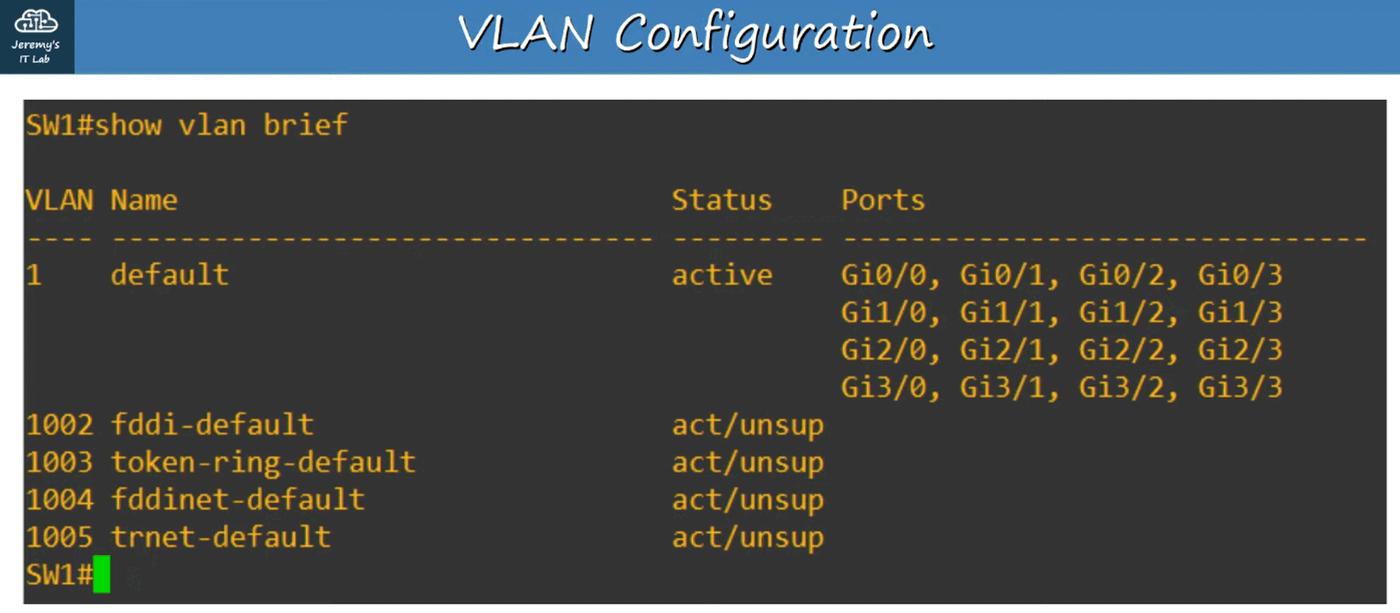
\includegraphics[keepaspectratio,alt={image}]{images/17-vlan-part1/img-010.png}}
\end{figure}

Shows which VLANS that exist on the SWITCH and what INTERFACES are in
each VLAN

VLANs 1 (DEFAULT), 1002-1005 exist by default and \textbf{cannot be
deleted (5 VLANs)}

\section{How to Assign Interfaces to a
VLAN}\label{how-to-assign-interfaces-to-a-vlan}

\begin{figure}
\centering
\pandocbounded{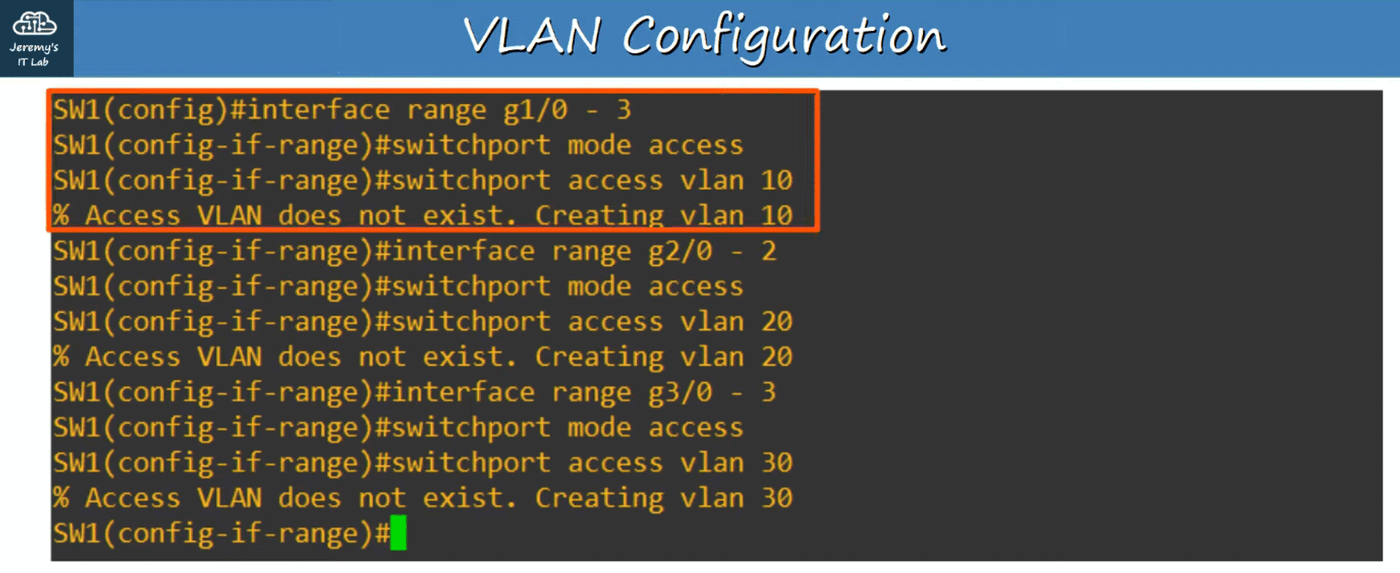
\includegraphics[keepaspectratio,alt={image}]{images/17-vlan-part1/img-011.png}}
\end{figure}

\begin{enumerate}
\def\labelenumi{\arabic{enumi})}
\item
  Use the ``interface range'' command to select all the interfaces at
  once
\item
  Use the ``switchport mode access'' command to set the interface as an
  ACCESS PORT
\end{enumerate}

WHAT IS AN ACCESS PORT?

\begin{itemize}
\tightlist
\item
  An ACCESS PORT is a SWITCHPORT which belongs to a single VLAN, and
  usually connects to end hosts like PCs.
\end{itemize}

SWITCHPORTS which carry multiple VLANs are called ``TRUNK PORTS'' (more
info on TRUNK in next chapter)

\begin{enumerate}
\def\labelenumi{\arabic{enumi})}
\setcounter{enumi}{2}
\tightlist
\item
  Use the ``switchport access'' command to assign a VLAN to a PORT
\end{enumerate}

\begin{figure}
\centering
\pandocbounded{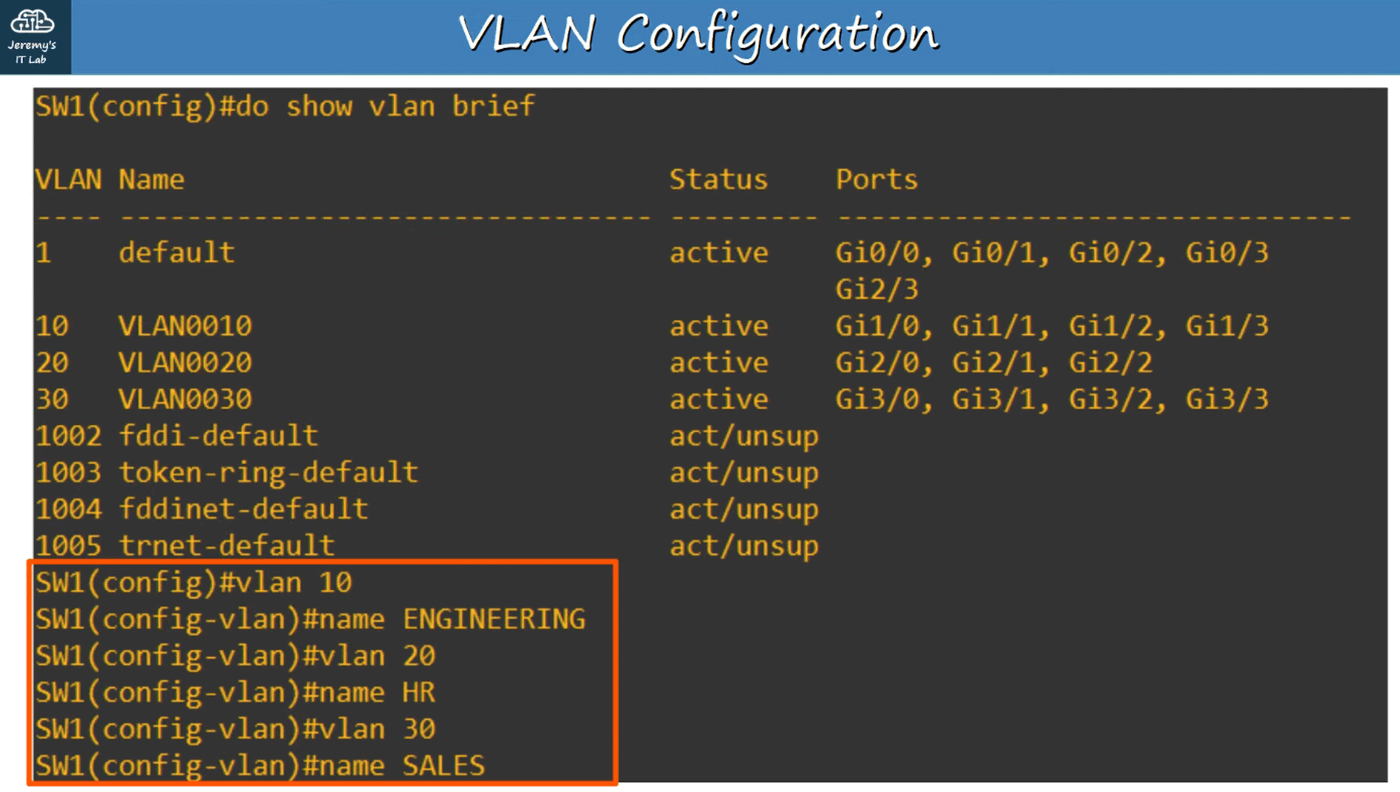
\includegraphics[keepaspectratio,alt={image}]{images/17-vlan-part1/img-012.png}}
\end{figure}

Use ``\#vlan \textless\#\textgreater'' to enter \textbf{Configuration
Mode} for a given VLAN (this can also create a VLAN)

Use ``\#name \textless name\textgreater'' to configure a NAME for your
VLAN

To check your VLAN configuration, use ``\#show vlan brief''

\begin{figure}
\centering
\pandocbounded{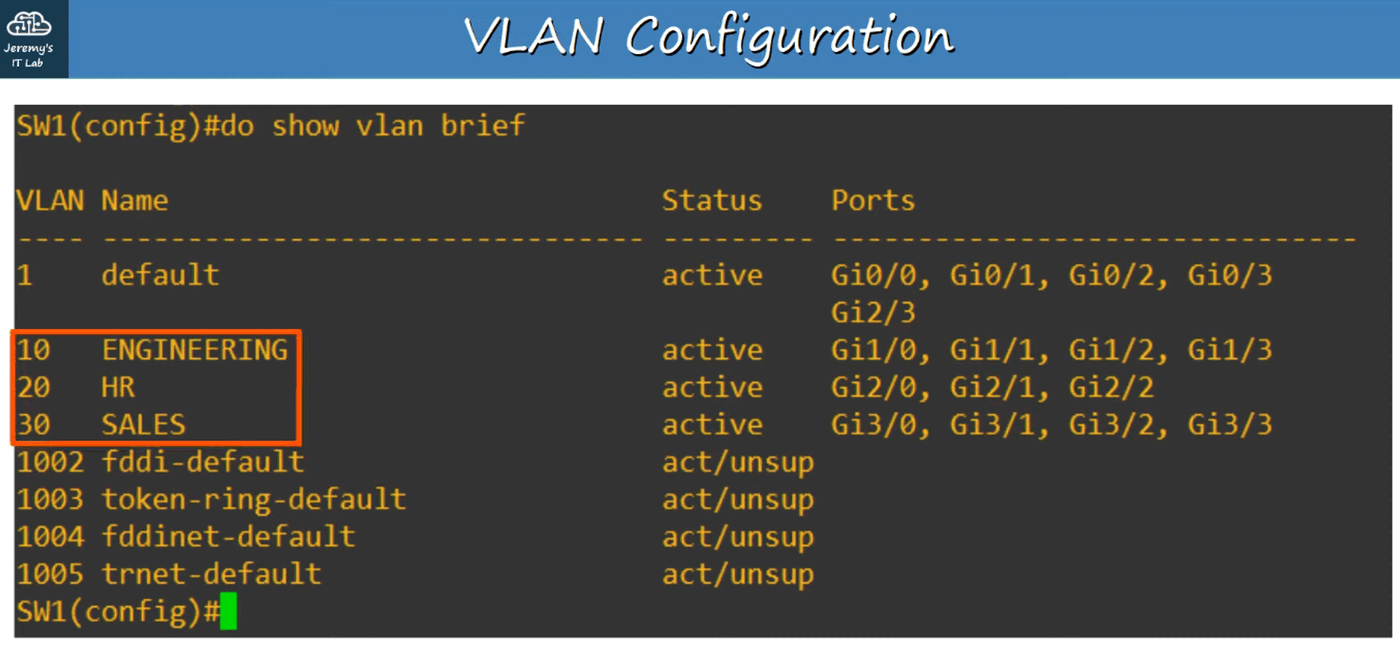
\includegraphics[keepaspectratio,alt={image}]{images/17-vlan-part1/img-013.png}}
\end{figure}

Testing VLAN 10

Pinging from PC1 using 255.255.255.255 (FFFF:FFFF:FFFF) floods broadcast
packets to R1 and VLAN10 hosts only

\begin{figure}
\centering
\pandocbounded{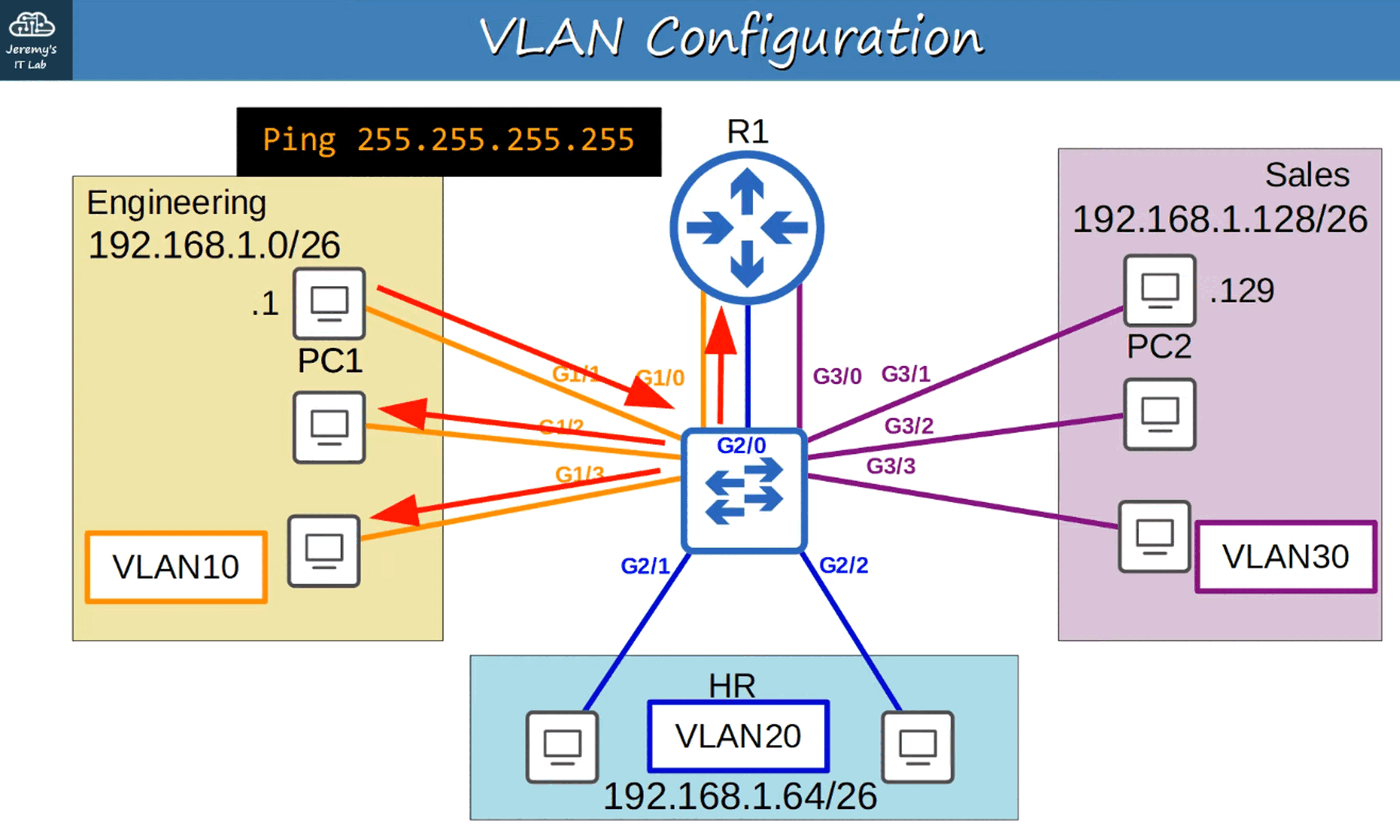
\includegraphics[keepaspectratio,alt={image}]{images/17-vlan-part1/img-014.png}}
\end{figure}
